\chapter{Telas do Programa}

Antes de detalhar as telas específicas, é importante compreender que a aplicação é construída sobre uma arquitetura modular de componentes. Cada tela é formada pela composição de múltiplos componentes reutilizáveis, que trabalham em conjunto para fornecer funcionalidades específicas:

\begin{itemize}
    \item \textbf{Componentes de Navegação}: Titlebar, breadcrumbs, botões de navegação
    \item \textbf{Componentes de Upload}: Área de drag-and-drop, seleção de arquivos, progresso
    \item \textbf{Componentes de Gerenciamento}: Seletores de coleção, editores, listas
    \item \textbf{Componentes de Visualização}: Viewers de coleção, imagem, gráficos e métricas
    \item \textbf{Componentes de Feedback}: Loading, popups
\end{itemize}

Esta arquitetura modular permite reutilização de código, manutenibilidade e consistência visual em toda a aplicação.

\section{Tela Principal}

A Tela Principal serve como ponto de entrada da aplicação e centro de controle para as principais operações. É a primeira interface que o usuário encontra ao abrir o programa.

\begin{figure}[H]
    \centering
    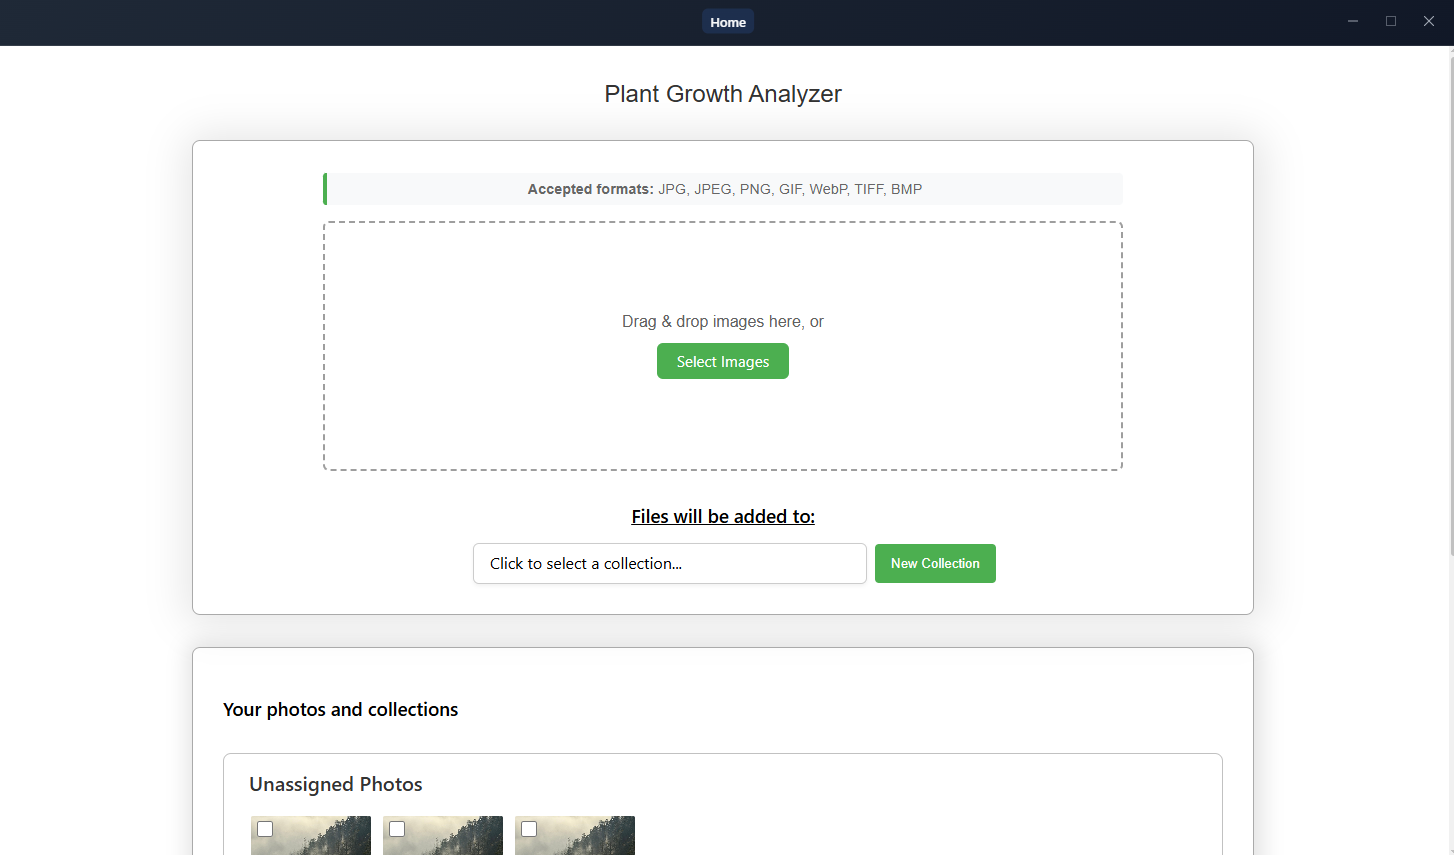
\includegraphics[width=0.9\textwidth]{../figures/hci/home_page.png}
    \caption{Tela Principal. Fonte: os autores}
    \label{fig:home-page}
\end{figure}


\section{Tela de Visualizar Coleção}

A Tela de Visualizar Coleção permite aos usuários explorar o conteúdo de uma coleção específica, visualizar as imagens processadas e analisar os dados de crescimento através de gráficos evolutivos.

\begin{figure}[H]
    \centering
    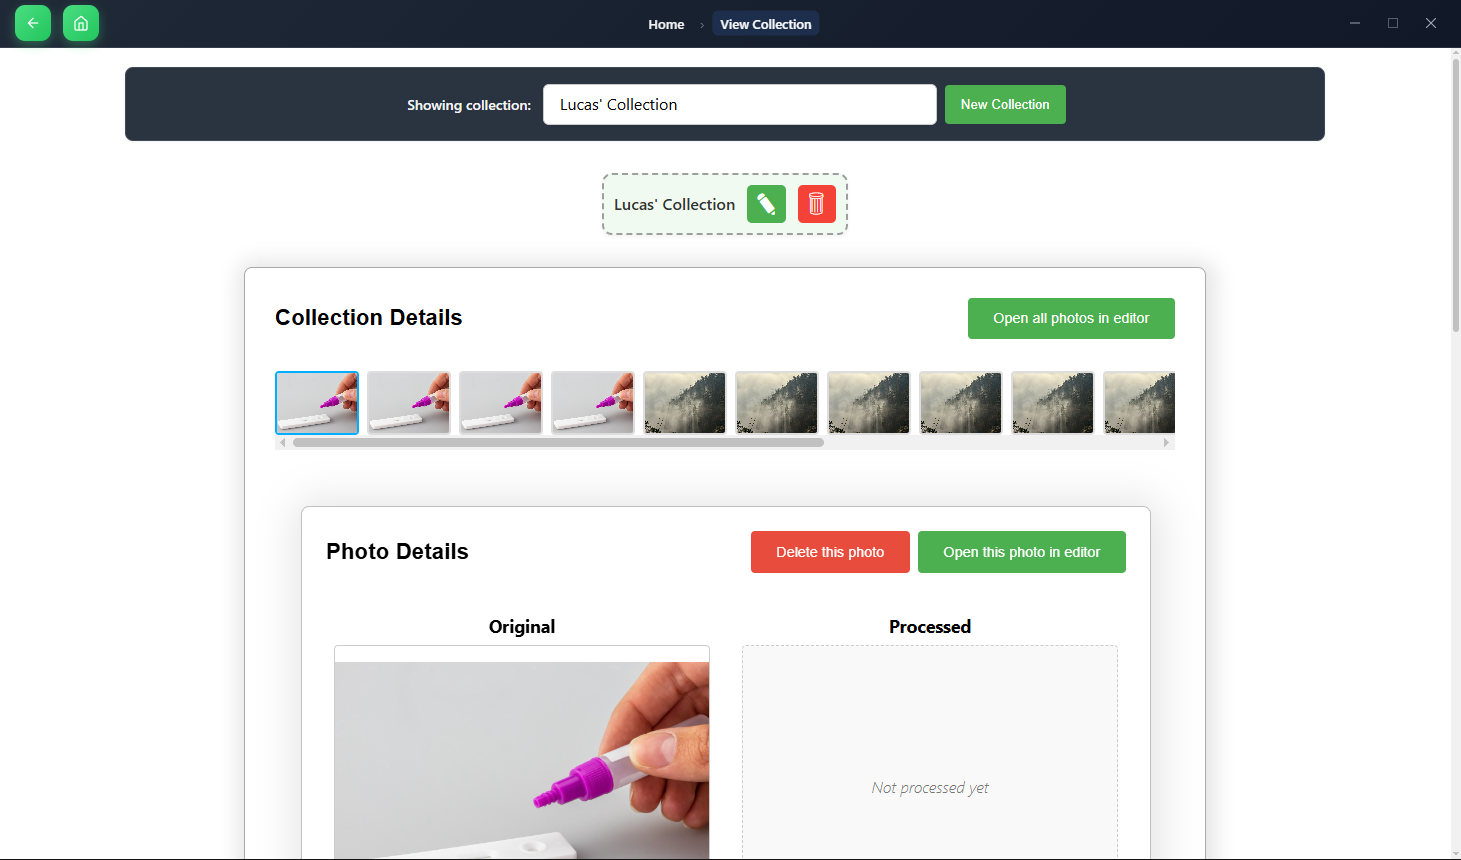
\includegraphics[width=0.9\textwidth]{../figures/hci/view_collection.png}
    \caption{Tela de Visualizar Coleção. Fonte: os autores}
    \label{fig:view-collection}
\end{figure}

\section{Tela de Visualizar Foto}

A Tela de Visualizar Foto oferece uma visualização detalhada de uma imagem específica, apresentando tanto a foto original quanto a versão processada, junto com as métricas extraídas.

\begin{figure}[H]
    \centering
    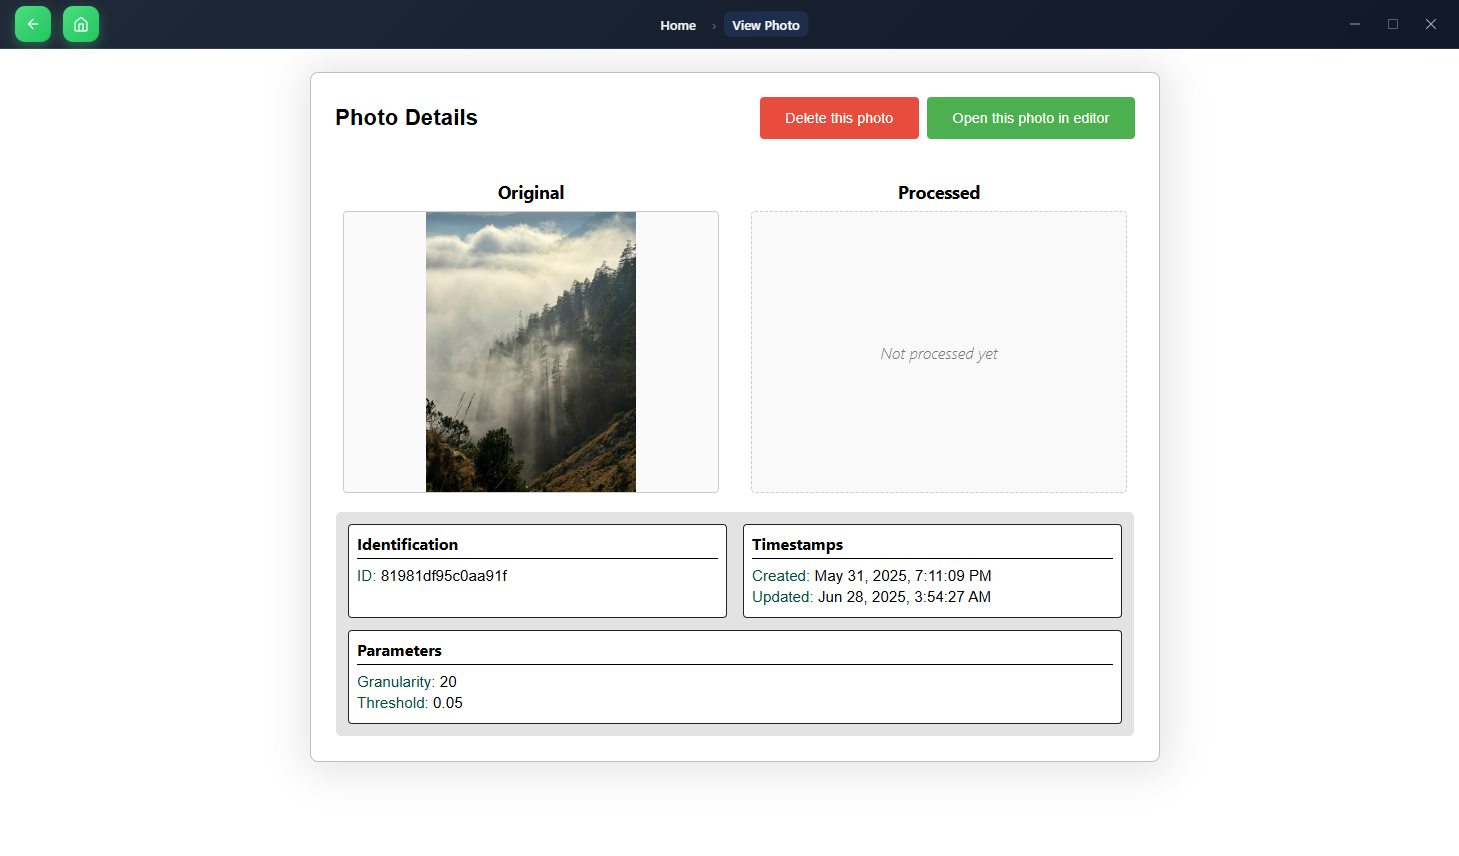
\includegraphics[width=0.9\textwidth]{../figures/hci/view_photo.png}
    \caption{Tela de Visualizar Foto. Fonte: os autores}
    \label{fig:view-photo}
\end{figure}

\section{Tela de Editar Foto}

A Tela de Editar Foto permite aos usuários ajustar configurações de processamento e metadados de uma imagem específica, oferecendo controle granular sobre o processo de análise.

\begin{figure}[H]
    \centering
    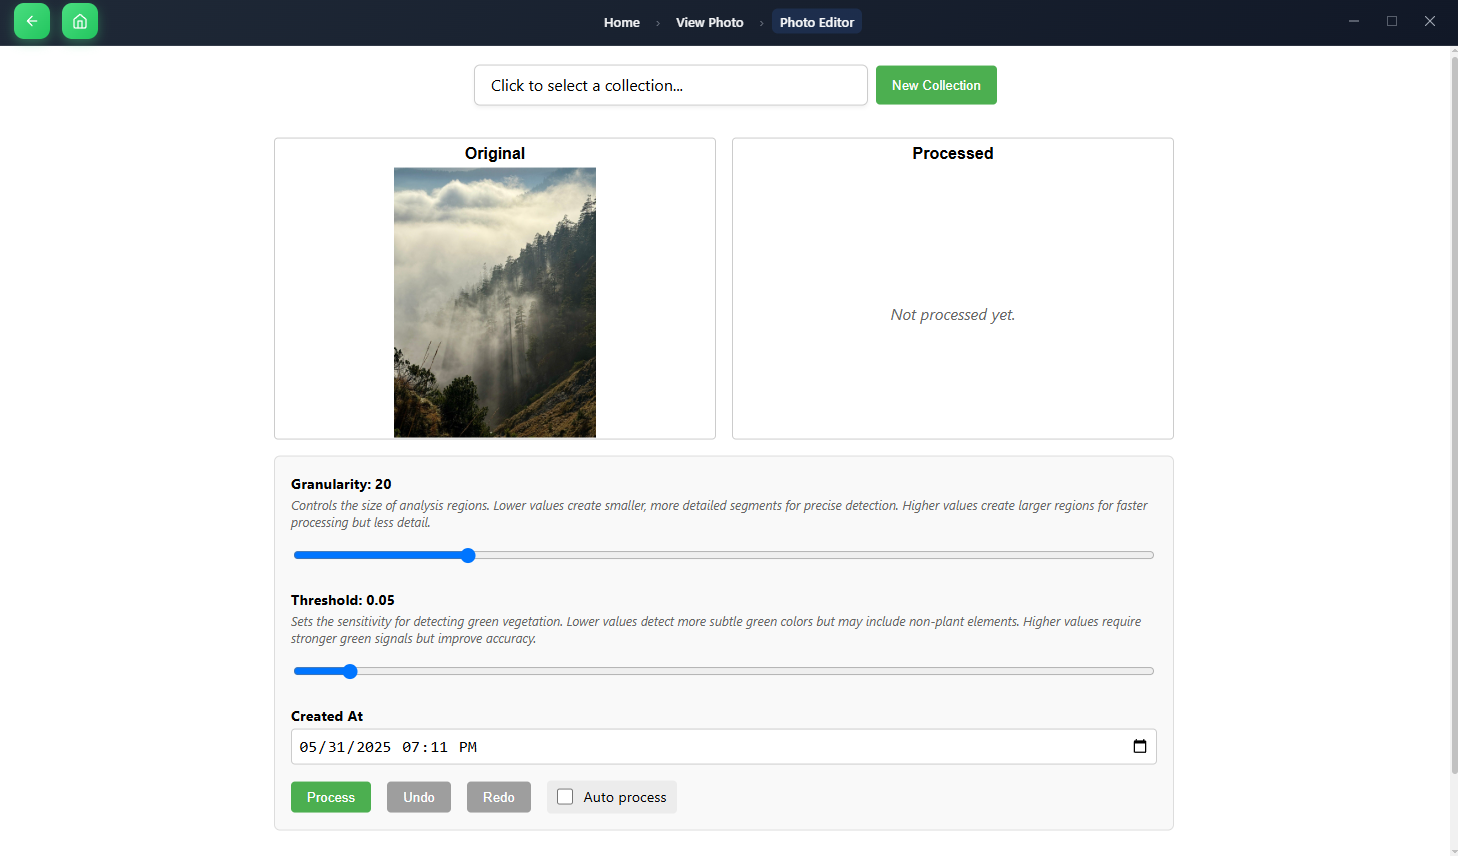
\includegraphics[width=0.9\textwidth]{../figures/hci/photo_editor.png}
    \caption{Tela de Editar Foto. Fonte: os autores}
    \label{fig:photo-editor}
\end{figure}

\section{Popups e Componentes Modais}

Além das quatro telas principais, a aplicação utiliza diversos popups e componentes modais para operações específicas e feedback ao usuário.

\subsection{Alguns exemplos}

\begin{enumerate}
    \item \textbf{Componente global de popups}
    \item \textbf{Componente global de loading/spinner}
    \item \textbf{Componente de edição flexível}: Muda sua estrutura visual dependendo da quantidade de fotos sendo processadas
\end{enumerate}
